%===================
% TODOs:
% Einzeilige Events, wenn Platz nicht reicht.

\documentclass[10pt,a4paper, landscape, ngerman]{article}
\usepackage[utf8]{inputenc}
\usepackage[left=2cm,right=2cm,top=2cm,bottom=2cm]{geometry}
\usepackage{babel}
\usepackage{translator}

\usepackage[T1]{fontenc}


\author{Tim Benedikt Herbstrith}
\pagestyle{empty}

\usepackage{tikz}
\usepackage{pgfcore}
\usepackage{pgfcalendar}
\usepackage{ifthen}


\usepackage{setspace}
\renewcommand{\arraystretch}{1.5}

\newcommand{\widthofday}{4}
\newcommand{\lengthofhour}{1}
\newcommand{\entrytextwidth}{3.5}

\newcommand{\firstH}{11}
\newcommand{\lastH}{19}


% Macro for drawing calendar entries
\newcommand{\calentry}[5]{
	\filldraw[black!20, rounded corners] ({day(#1,-1)},{time(#2)}) rectangle ({day(#1,1)},{time(#3)});%
	\node[anchor=north, font=\scriptsize, text width=\entrytextwidth cm] at ({day(#1,0)},{time(#2)}) {#2\\ \textbf{#4}\\ #5};%
}
\newcommand{\shortcalentry}[4]{
	\filldraw[black!20, rounded corners] ({day(#1,-1)},{time(#2)}) rectangle ({day(#1,1)},{time(#3)});%
	\node[font=\scriptsize, text width=\entrytextwidth cm] at ({day(#1,0)},{halftime(#2,#3)}) {\textbf{#4}};%
}
%\newcommand{\entry}[5]{%
%	\ifthenelse{\equal{\isshort{#2}{#3}}{0.0}}{%
%		\calentry{#1}{#2}{#3}{#4}{#5}%
%	}{%
%		\shortcalentry{#1}{#2}{#3}{#4}%
%	}%
%}

%% Determine, whether event is too short to print whole information.
%\newcommand{\isshort}[2]{%
%	\pgfmathlessthan{#2-#1}{0.75}
%	\pgfmathresult
%}

\begin{document}
\begin{center}

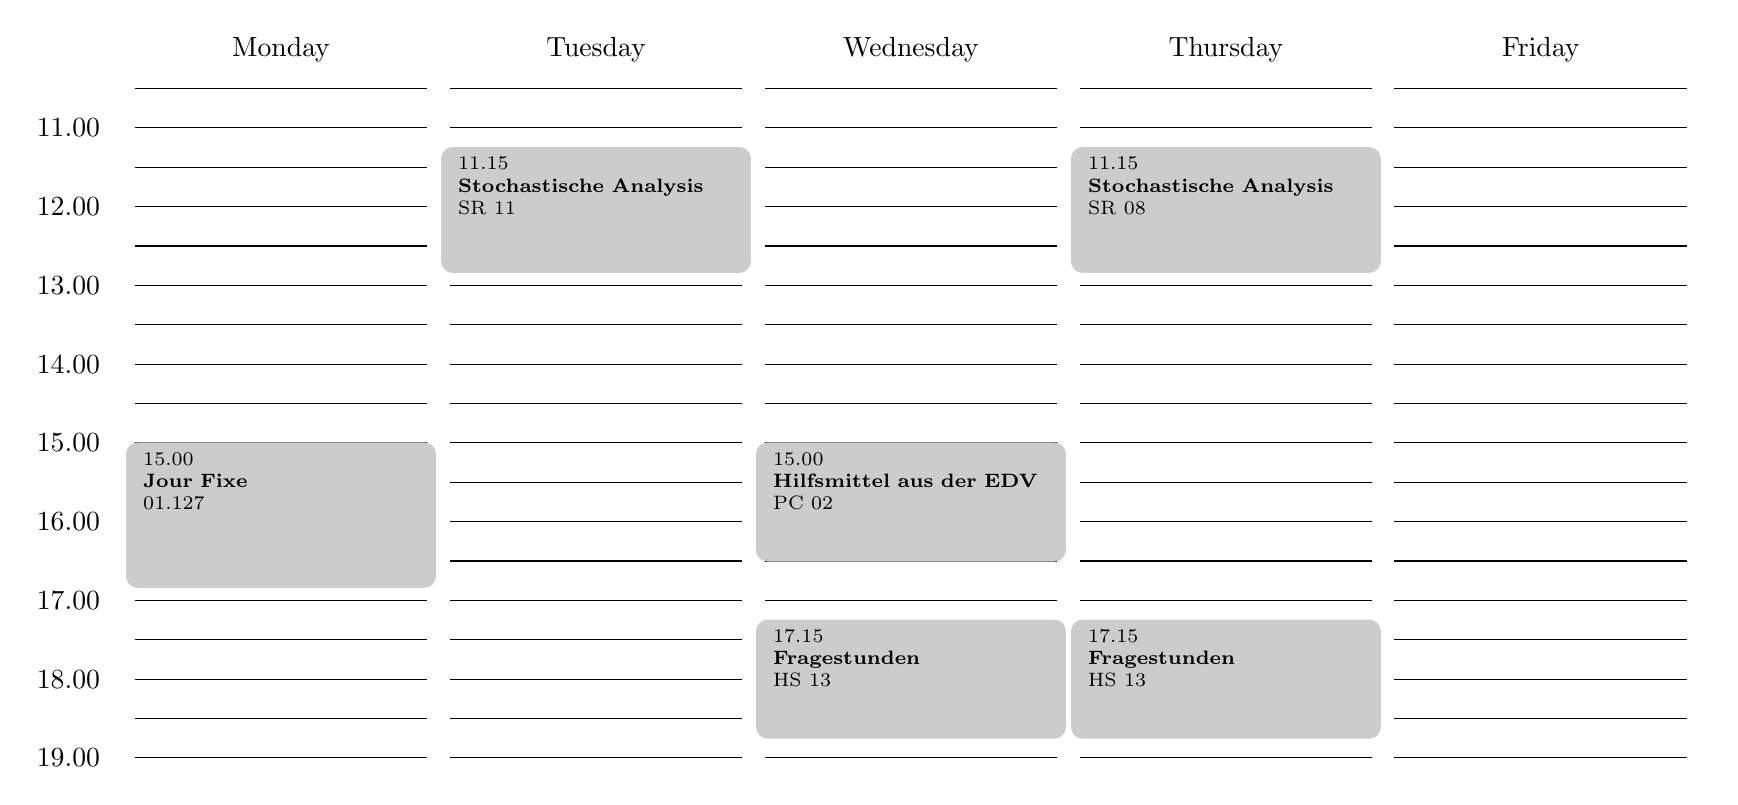
\begin{tikzpicture}[x=\widthofday cm, y=\lengthofhour cm]

% Offset for the rectangle marking appointments
\pgfmathsetmacro{\offsetForAppointment}{+0.01}

% Converts the integer marking the day of the week to a coordinate.
% The second argument specifies wheter the left (-1), the base (0) or the right end of the column is returned.
\pgfmathdeclarefunction{day}{2}{%
	\pgfmathparse{-#2*\offsetForAppointment+#1-(1-#2)/2}%
}

% Converts a given time (hh.mm) to a length. \firstH is converted to 0.
\pgfmathdeclarefunction{time}{1}{%
	\pgfmathparse{\firstH-(floor(#1)+(#1-floor(#1))/0.6)}%
}
\pgfmathdeclarefunction{halftime}{2}{%
	\pgfmathparse{(time(#1)+time(#2))/2}%
}
	
\foreach \hour in {\firstH,...,\lastH}
	\draw (0,\firstH-\hour) node[left=5] {\hour.00} -- (5,\firstH-\hour)  (0,\firstH+0.5-\hour) -- (5,\firstH+0.5-\hour);
\foreach \day in {0,...,5}
	\draw[line width=8pt,white] (\day,0.6) -- (\day,\firstH-\lastH -0.1);
\foreach \day in {0,...,4}
	\node at (0.5+\day,1) {\pgfcalendarweekdayname{\day}};
	
\calentry{1}{15.00}{16.50}{Jour Fixe}{01.127}
\calentry{2}{11.15}{12.50}{Stochastische Analysis}{SR 11}
\calentry{3}{15.00}{16.30}{Hilfsmittel aus der EDV}{PC 02}
\calentry{3}{17.15}{18.45}{Fragestunden}{HS 13}
\calentry{4}{17.15}{18.45}{Fragestunden}{HS 13}
\calentry{4}{11.15}{12.50}{Stochastische Analysis}{SR 08}

\end{tikzpicture}

\end{center}
\end{document}